% !TEX program = xelatex
% ¡Recuerda compilar con XeLaTeX o LuaLaTeX!
\documentclass{article}

% --- Cargar nuestro fichero de estilo ---
% Se asume que paper_style.sty está disponible o se usan paquetes estándar.
\usepackage{paper_style}

% --- PAQUETES PARA EL CONTENIDO DEL DOCUMENTO ---
\usepackage{graphicx}
\usepackage{subcaption}
\usepackage{amsmath}
\usepackage{booktabs}
\usepackage{geometry}
\usepackage{hyperref}
\usepackage{enumitem}
\usepackage{float}


% --- Cambiar numeración de subsecciones ---
\renewcommand{\thesubsection}{\alph{subsection})}


% --- Información del Paper ---
\title{Práctica 3: \\ Análisis de Accesibilidad de UACLOUD}
\author{
	Jordi Blasco Lozano \\
	\small Interacción Persona Máquina
	\small Universidad de Alicante
}
\date{\today}

% --- Comienzo del Documento ---
\begin{document}
	
	\maketitle

	\begin{abstract}
	\noindent Para la evaluación de la accesibilidad de la plataforma UACLOUD, utilicé el lector de pantalla Narrador de Windows. El análisis se ha centrado en la funcionalidad de dos de las aplicaciones internas:  \textbf{a) Deportes} y \textbf{b) Horarios}, revelando los problemas de accesibilidad críticos que impiden su uso a personas dependientes de esta tecnología de asistencia.
	\end{abstract}



	\section{Análisis de Accesibilidad de la Plataforma UACLOUD con Lector de Pantalla}

    

	\subsection{Evaluación de la Aplicación de Deportes: Reserva de Pista de Pádel}

	La experiencia en la aplicación de Deportes presenta una accesibilidad deficiente que frustra por completo el proceso de reserva de una pista de pádel.	Aunque la navegación inicial hasta la sección de ``Pádel'' es relativamente intuitiva, el flujo de reserva es impracticable para un usuario de lector de pantalla. Los principales problemas detectados son:

	\begin{itemize}
		\item \textbf{Estructura y navegación no jerárquicas}: Al llegar a la selección de hora, la página carece de una estructura jerárquica clara. El usuario no recibe indicaciones sobre si debe navegar con el tabulador o las teclas de flecha, lo que requiere una memorización previa de la interfaz para poder interactuar con ella, incumpliendo el criterio \textbf{WCAG 2.4.3 Orden del foco}.

		\item \textbf{Controles no operables}: Los elementos para cambiar de día (las flechas de navegación) no están correctamente implementados. El lector de pantalla los anuncia, pero no son activables mediante el teclado, lo que limita la reserva exclusivamente al día actual.

		\item \textbf{Fallos en la confirmación}: Al seleccionar un horario y aparecer el panel para elegir una pista individual o doble, el botón de confirmación ("90 min") es completamente inaccesible. No puede ser enfocado ni activado mediante ninguna combinación de teclas (espacio, intro, flechas), ya que la acción asociada al control no es reconocida por el Narrador. Esto incumple el criterio \textbf{WCAG 2.1.1 Teclado} y \textbf{WCAG 4.1.2 Nombre, función, valor}, ya que los componentes no exponen su funcionalidad a las tecnologías de asistencia.
	\end{itemize}

	La herramienta de evaluación automática \textbf{Accessibility Insights} corrobora parcialmente estos hallazgos. Si bien no detecta los controles inoperables, sí identifica correctamente:
	\begin{itemize}
		\item \textbf{Contraste de color insuficiente}: Reporta 41 elementos en la interfaz de horarios con un bajo contraste, dificultando la lectura para usuarios con baja visión (\textbf{WCAG 1.4.3 Contraste Mínimo}).
		\item \textbf{Orden de tabulación deficiente}: Confirma que el orden de foco no es lógico ni predecible.
		\item \textbf{Falta de etiquetas (labels)}: Detecta múltiples elementos interactivos que carecen de una descripción textual accesible, impidiendo que el usuario sepa su propósito (\textbf{WCAG 4.1.2 Nombre, función, valor}).
	\end{itemize}

	\subsection{Evaluación de la Aplicación de Horarios}

	La aplicación de Horarios presenta barreras de accesibilidad aún más severas que la de Deportes, resultando completamente inutilizable.

	La principal deficiencia reside en la \textbf{tabla de horarios}, que es totalmente inoperable. A diferencia de la aplicación de Deportes, donde al menos era posible interactuar con algunos elementos, aquí es imposible acceder o interpretar la información del horario.

	\begin{itemize}
		\item \textbf{Lectura incorrecta de la tabla}: Al intentar navegar por la tabla, el Narrador de Windows se limita a verbalizar las coordenadas de las celdas vacías (por ejemplo, "fila dos de treinta y dos, columna uno de dos"), sin leer en ningún momento el contenido real de las mismas. Esto indica una implementación incorrecta de la tabla, que carece de la semántica necesaria para que las tecnologías de asistencia la interpreten, incumpliendo el criterio \textbf{WCAG 1.3.1 Información y relaciones}.

		\item \textbf{Etiquetas incorrectas o ausentes}: Los botones y otros controles interactivos poseen etiquetas que no se corresponden con su función real, generando una gran confusión y haciendo imposible la navegación con certeza.
	\end{itemize}

	Según la herramienta automática, esta página presenta menos problemas de \textbf{contraste de color} (aproximadamente la mitad que la aplicación de Deportes) y, curiosamente, no detecta errores significativos en el \textbf{orden de tabulación}. Sin embargo, a pesar de estos resultados, la experiencia manual demuestra que la aplicación es totalmente inaccesible debido a los fallos estructurales y de etiquetado que impiden al lector de pantalla cumplir su función.

	\section{Anexos: Capturas de Pantalla
	}
		\begin{figure}[H]
		\centering
		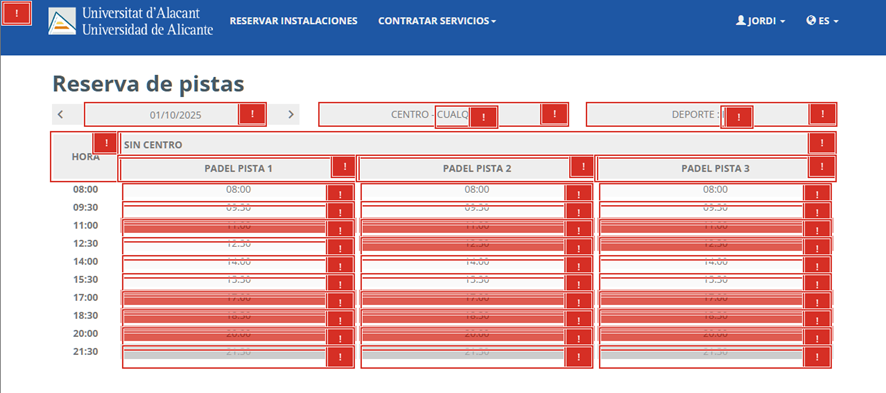
\includegraphics[width=\textwidth]{horario_padel_contrastes.png}
		\caption{Análisis de contrastes en la reserva de pistas de pádel.}
		\label{fig:deportes_insights}
	\end{figure}

	\begin{figure}[H]
		\centering
		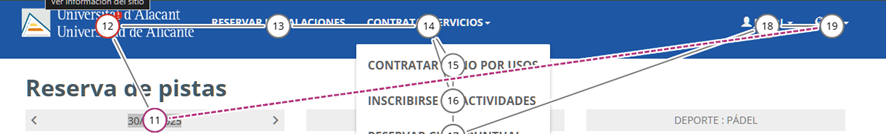
\includegraphics[width=\textwidth]{padel_tabulaciones.png}
		\caption{Análisis de tabulaciones en la reserva de pistas de pádel.}
		\label{fig:deportes_eyetracking}
	\end{figure}

	\begin{figure}[H]
		\centering
		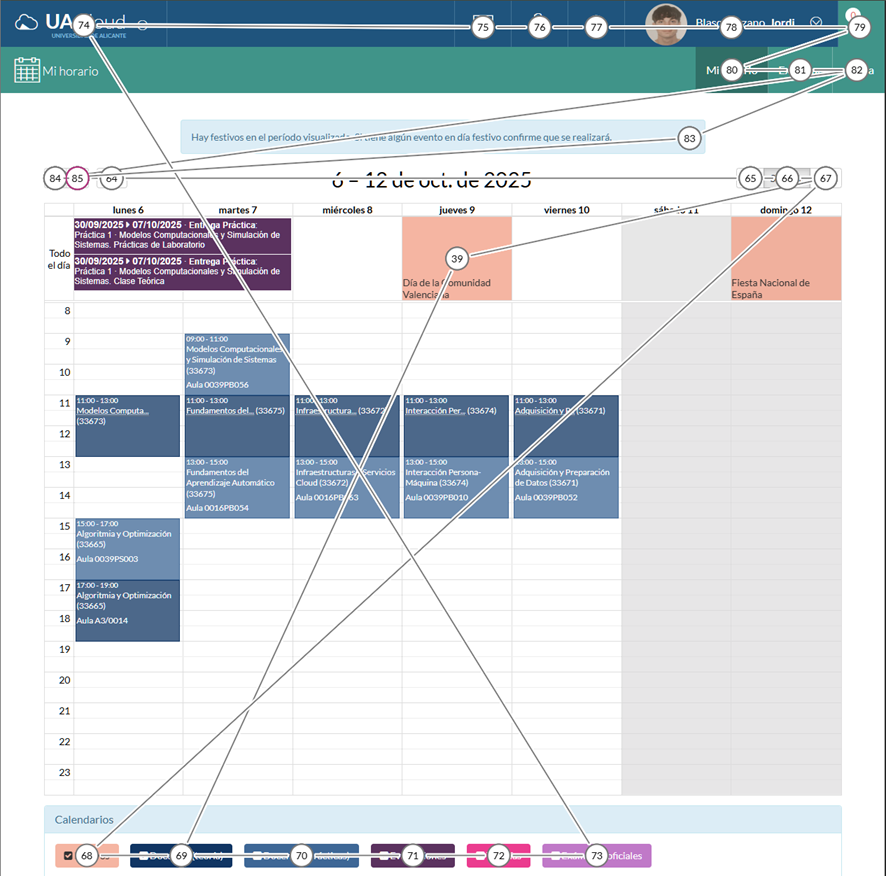
\includegraphics[width=\textwidth]{hoario_tabulaciones.png}
		\caption{Análisis de tabulaciones en la aplicación de Horarios.}
		\label{fig:horarios}
	\end{figure}



\end{document}